\documentclass[11pt,letterpaper]{article}
\PassOptionsToPackage{hyphens}{url}
\usepackage[margin=.83in,top=.8in,bottom=.8in,headheight=15pt]{geometry}
\usepackage[T1]{fontenc}
\usepackage{lmodern,amsmath,amssymb,mathtools,bm,booktabs,array,graphicx,tikz}
\usetikzlibrary{arrows.meta,positioning,calc,decorations.pathreplacing,patterns}
\definecolor{ink}{HTML}{17344D}\definecolor{accent}{HTML}{087E8B}\definecolor{pale}{HTML}{EDF5F5}\definecolor{gold}{HTML}{AD6B19}
\providecommand{\dd}{\,\mathrm{d}}\providecommand{\R}{\mathbb{R}}
\providecommand{\E}{\mathbb{E}}\providecommand{\Var}{\operatorname{Var}}
\providecommand{\Cov}{\operatorname{Cov}}\providecommand{\diag}{\operatorname{diag}}
\providecommand{\norm}[1]{\left\lVert#1\right\rVert}
\providecommand{\abs}[1]{\left|#1\right|}
\usepackage{microtype,hyperref,fancyhdr,enumitem,amsthm,sectsty,needspace}
\allsectionsfont{\raggedright}
\hypersetup{colorlinks=true,linkcolor=ink,urlcolor=accent,pdfauthor={Zan Ahmad},pdftitle={Cardiac phase and pressure feedback in a pulsatile circulation / Lecture notes}}
\setlength{\parindent}{0pt}\setlength{\parskip}{6pt}\linespread{1.07}
\setlist{itemsep=3pt,topsep=4pt,leftmargin=*}
\emergencystretch=2em\clubpenalty=10000\widowpenalty=10000
\pagestyle{fancy}\fancyhf{}\fancyhead[L]{\small Computational Cardiology}\fancyhead[R]{\small Lecture 4}
\fancyfoot[L]{\footnotesize Zan Ahmad}\fancyfoot[R]{\footnotesize\thepage}\renewcommand{\headrulewidth}{.3pt}
\newtheorem{proposition}{Proposition}\newtheorem{theorem}{Theorem}\newtheorem{lemma}{Lemma}
\theoremstyle{definition}\newtheorem{definition}{Definition}\newtheorem{example}{Example}
\numberwithin{equation}{section}
\begin{document}
{\small\scshape Computational Cardiology\hfill Lecture 4}\par\medskip
{\raggedright\hyphenpenalty=10000\exhyphenpenalty=10000\LARGE\bfseries\color{ink} Cardiac phase and pressure feedback in a pulsatile circulation\par}\medskip
{\small Lecture notes}\par\bigskip
Pressure regulation couples a slow measurement filter to the phase of a pulsatile pump. The clock must accumulate heart rate, while the hydraulic equations must conserve the stored blood volume. These two couplings distinguish a continuously varying rate from merely replacing the frequency in a fixed-rate formula.

\section{The circulation boundary and constitutive laws}
\hypertarget{note-the-circulation-boundary-and-constitutive-laws}{}\label{note:the-circulation-boundary-and-constitutive-laws}
{\small \href{slides.html\#frame=storage-and-boundary-conditions-figure\&step=1}{Slides for this section}}\par
Our plant is a closed six-compartment circulation: left ventricle, systemic arteries, systemic veins, right ventricle, pulmonary arteries and pulmonary veins. Four ideal one-way valves connect the ventricles to the adjacent vessels; systemic and pulmonary resistance beds connect arteries to veins. These beds permit signed flow according to their pressure difference. Every transfer leaves one compartment and enters another. No blood enters from a prescribed external atrium, and no blood disappears into an outlet reservoir. This boundary determines a nonnegotiable test: the total blood volume stays constant.

Each compartment has an unstressed volume plus a pressure-dependent stored volume. Vascular compliance is constant in this model, while ventricular compliance follows a periodic contraction--relaxation waveform. The two ventricles use one cardiac phase, although their compliance endpoints differ. Pressure is in mmHg, volume in litres, and hydraulic time in minutes. Resistance therefore has units mmHg min/L and compliance has units L/mmHg. The interface displays seconds; every hydraulic step converts seconds to minutes. Naming this conversion prevents a factor-of-60 error that can otherwise look like a strong physiological effect.

The public companion paper provides an instructive contrast: it stores blood in a left ventricle and a systemic artery, with an external fixed-pressure inlet and an outlet reservoir. Its feedback loop is closed, but its stored blood volume need not be constant. A result can be correct for that boundary and wrong for this one. Before transferring any published graph, identify its compartments, reservoirs, controlled variable and forcing. Here the controlled signal is filtered systemic arterial pressure; systemic resistance is the imposed disturbance, and heart rate is the actuator.

The model omits atrial contraction, baroreceptor dynamics beyond a single filter, oxygen demand, vascular adaptation and spatial pressure waves. Consequently, calling the resistance interval ``exercise'' is a protocol label, not a complete model of exercise. It is useful precisely because we can isolate one proposed mechanism. Ask whether that mechanism produces the intended qualitative response while satisfying the accounting, rather than whether a familiar-looking plot is enough to establish realism.

\[
V_i=V_{d,i}+C_iP_i,\qquad Q_{ij}=\frac{P_i-P_j}{R_{ij}}
\]
V in L, C in L/mmHg, P in mmHg and Q in L/min. For an ideal valve, replace the signed pressure difference by its positive part.

The open two-storage model in Ahmad and Peskin's feedback paper and the closed six-storage companion have different blood-flow boundaries. For the former, summing storage gives $\dot x_{LV}+\dot x_A=Q_{Mi}-Q_s$. For the latter, every transfer is internal and $\sum_i\dot V_i=0$. Closing the feedback signal path does not itself close the blood circuit.

\paragraph{Calculation.} A closed ventricle has C\_old = 0.010 L/mmHg, P\_old = 8 mmHg and C\_new = 0.005 L/mmHg. What pressure preserves its stored volume?

Its old stressed volume is 0.010 \ensuremath{\times} 8 = 0.080 L.

Closed valves give zero net transfer, so C\_new \ensuremath{\times} P\_new must equal 0.080 L.

Divide by the new compliance: P\_new = 0.080/0.005 = 16 mmHg.

Pressure doubles while volume stays constant. Updating P as though C were fixed would miss this response.
\begin{center}\begin{minipage}{.98\linewidth}\centering
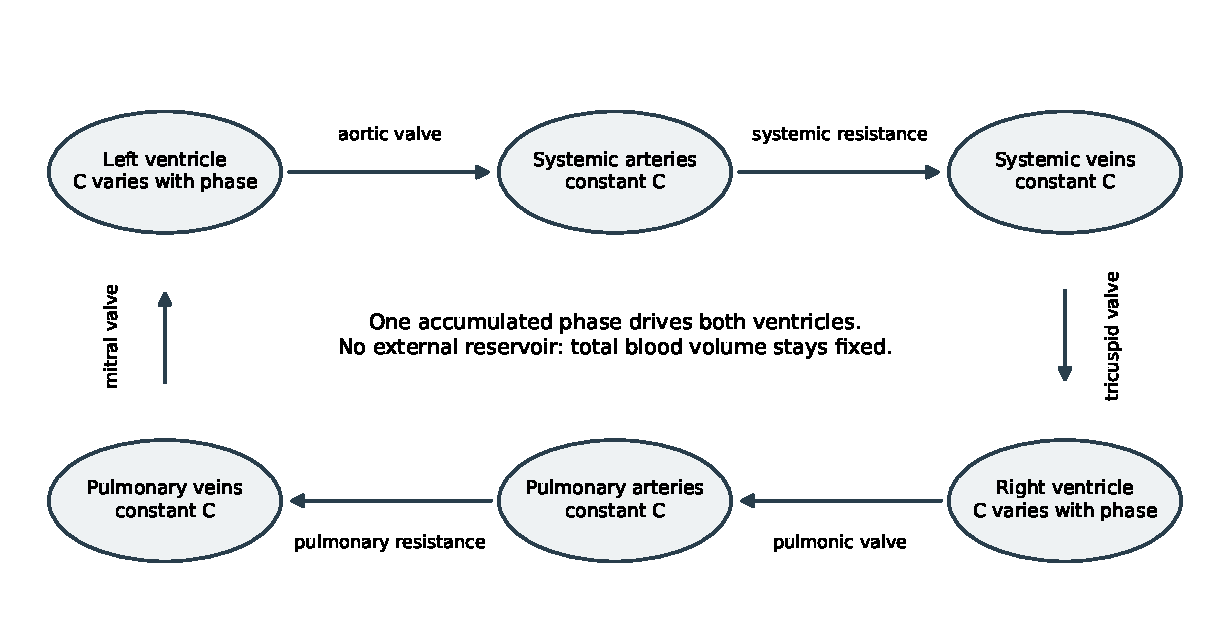
\includegraphics[width=.96\linewidth,height=.57\textheight,keepaspectratio]{circuit.pdf}\par\smallskip
{\small Original schematic of the model boundary and flow connections. Four ideal valves enforce direction; resistance beds use signed pressure-driven flow. Both ventricular compliances share one phase.}
\end{minipage}\end{center}
\section{Conservative implicit hydraulics}
\hypertarget{note-conservative-implicit-hydraulics}{}\label{note:conservative-implicit-hydraulics}
{\small \href{slides.html\#frame=the-implicit-hydraulic-step\&step=1}{Slides for this section}}\par
For a changing compliance, the pressure derivative alone is not the storage derivative. Apply conservation to the product C P. Expanding that product produces a term P times the compliance derivative. Dropping it erases the pumping mechanism: the ventricle can change pressure even when its valves are closed, because its compliance changes at fixed volume. We therefore discretize the stored product directly. With step h in minutes, the new stored volume equals the old stored volume plus h times the net new flow.

Hold a candidate valve configuration fixed for a moment. Every open connection contributes a conductance G = 1/R. Its contribution to the pressure matrix is hG on two diagonal entries and \ensuremath{-}hG on the paired off-diagonal entries. The resulting conductance Laplacian L has zero row and column sums. Adding the new positive compliances on the diagonal yields a symmetric positive-definite matrix for this connected passive network with positive storage. Solve the six-by-six linear system; do not explicitly invert its matrix.

Now inspect the resulting pressure order at each valve. An open valve must have upstream pressure at least downstream pressure; a closed valve must have the opposite order, allowing equality. If the candidate violates these conditions, update its state and solve again. The companion caps iteration and, if necessary, checks the sixteen possible four-valve configurations. A failure to find a consistent configuration raises an error instead of silently accepting a last iterate. A small linear residual without valve consistency is not a valid nonlinear step.

Multiply the accepted matrix equation by the all-ones row vector. The Laplacian contribution vanishes, leaving equality of the old and new sums of C P. Constant unstressed volumes then give conservation of total blood volume. This proof explains the diagnostic; it does not prove temporal accuracy. A coarse step can conserve volume perfectly while shifting valve-opening times and distorting pressure extrema. We must check the balance, the valve conditions and refinement separately.

\[
\frac{d(C_iP_i)}{dt}=\sum_j Q_{ji}-\sum_j Q_{ij}
\]


\[
\left[\operatorname{diag}(C^{n+1})+hL(S^{n+1},R^{n+1})\right]P^{n+1}=C^n\mathbin{\odot}P^n
\]
S denotes valve states. The pressure solve is implicit; hG and C both have units L/mmHg.

\[
\sum_i(V_{d,i}+C_i^{n+1}P_i^{n+1})=\sum_i(V_{d,i}+C_i^nP_i^n)
\]


Changing ventricular compliance is an energy input to the hydraulic model. In an isolated chamber,
\[
 \dot P=-\frac{\dot C}{C}P.
\]
A decrease in compliance raises pressure at fixed stored volume. The pressure solver must therefore use $C^{n+1}P^{n+1}-C^nP^n$, including the compliance change before deciding which valves conduct.

\paragraph{Calculation.} Trace a valve-state correction in a deliberately reduced two-compartment problem. Both compliances are 0.010 L/mmHg; old pressures are 20 and 10 mmHg. A single ideal valve permits flow from A to B with resistance 1 mmHg min/L. There are no other connections, compliances stay fixed, and h = 0.010 min. This small reduction illustrates the active-valve solve; it is not the two-compartment reservoir model in the reading.

Guess the valve is closed. With no flow and unchanged compliance, the candidate new pressures are still PA = 20 and PB = 10 mmHg. This state conserves total stressed volume, 0.300 L, but fails the closed-valve condition because PA > PB.

Revise the guess to open. Here h/R = 0.010 L/mmHg. The pressure matrix has diagonal entries 0.020 and off-diagonal entries \ensuremath{-}0.010 L/mmHg; the right-hand side is [0.200, 0.100] L.

Divide both equations by 0.010 L/mmHg: 2 PA \ensuremath{-} PB = 20 mmHg and \ensuremath{-}PA + 2 PB = 10 mmHg. Solving gives PA = 50/3 = 16.6667 mmHg and PB = 40/3 = 13.3333 mmHg.

The revised pressure difference is 10/3 mmHg, so the accepted forward flow is Q = 10/3 = 3.3333 L/min. PA > PB agrees with the open guess. The transferred volume is hQ = 1/30 = 0.0333333 L.

Compartment A changes from 0.200 to 1/6 = 0.166667 L; B changes from 0.100 to 2/15 = 0.133333 L. Their sum remains 0.300 L. Both conservation and valve consistency now pass.

Reject the closed candidate despite its correct total volume. Accept the open candidate only after checking its pressure ordering and compartment transfers.
\section{Filtered pressure and bounded proportional control}
\hypertarget{note-filtered-pressure-and-bounded-proportional-control}{}\label{note:filtered-pressure-and-bounded-proportional-control}
{\small \href{slides.html\#frame=filter-the-arterial-pressure\&step=1}{Slides for this section}}\par
Arterial pressure pulsates within each beat. Directly commanding the heart rate from the instantaneous waveform would feed this fast oscillation back into the clock. The pressure filter introduces a separate state that follows arterial pressure over a time scale tau. The companion uses forward Euler: the next filtered pressure is a weighted combination of the old filtered value and the old arterial pressure. The code requires 0 < step/tau \ensuremath{\le} 1, which keeps this filter update between those two inputs. The broader linear stability interval is not the same as this non-overshooting condition.

Define a positive dimensionless gain g. A filtered pressure below the positive target gives a positive relative error and raises the rate command. A filtered pressure above target lowers it. The original assignment uses a negative gain c multiplying the reversed pressure error; the two conventions agree when g = \ensuremath{-}c. Check the sign with a deliberately low pressure before running a long simulation. Gain has no time units here because the pressure error is normalized by its target and multiplied by the reference rate.

A proportional controller does not automatically remove steady error. In an operating regime requiring a higher rate than the reference, the algebraic controller generally needs a persistent pressure error to command that higher rate. A residual offset is therefore not by itself evidence of a coding mistake. Increasing gain may reduce the offset but changes transient dynamics and can drive the command into saturation. Our explicit lower and upper rate bounds keep the cardiac phase advancing; they also change the model whenever active. Record the unbounded command alongside the bounded rate so saturation remains visible.

The current public paper also presents an exponential held-input filter. That formula integrates the filter exactly over a step if the arterial pressure is held fixed during that step. It is useful for a method comparison, but it does not make the coupled circulation integrator exact or second order. The companion retains the Euler method specified by the historical project; the held-input exponential update is a distinct available comparison.

\[
p_f^{n+1}=p_f^n+\frac{\Delta t}{\tau}(P_{sa}^n-p_f^n)
\]
Use the same time units for step and tau; the implementation uses seconds for this ratio.

\[
F_{\rm cmd}=F_0\left[1+g\frac{P_*-p_f^{n+1}}{P_*}\right],\qquad F=\min(F_{\max},\max(F_{\min},F_{\rm cmd}))
\]
The target P\_* must be positive. The implemented default gain is 10; it is an illustrative choice, not a fitted parameter.

For pressure held constant during an interval, the filter equation has the exact solution
\[
 \bar P(t+h)=P_a+\bigl(\bar P(t)-P_a\bigr)e^{-h/\tau}.
\]
The implemented forward-Euler filter instead uses $\bar P^{n+1}=(1-h/\tau)\bar P^n+(h/\tau)P_a^n$. It is a convex combination for $0\le h/\tau\le1$. The held-input solution explains the relaxation time but is not a claim that the companion uses that update.

\paragraph{Calculation.} Take filtered pressure 90 mmHg, arterial pressure 80 mmHg, step 0.0075 s, tau 3 s, target 90 mmHg, reference rate 80 beats/min and gain 5.

The filter weight is 0.0075/3 = 0.0025.

The next filtered pressure is 90 + 0.0025 \ensuremath{\times} (80 \ensuremath{-} 90) = 89.975 mmHg.

The command is 80 \ensuremath{\times} [1 + 5 \ensuremath{\times} (90 \ensuremath{-} 89.975)/90] = 80.1111 beats/min.

The rate rises slightly, with no saturation. A pressure deficit must not lower the rate under this convention.
\section{The accumulated cardiac clock}
\hypertarget{note-the-accumulated-cardiac-clock}{}\label{note:the-accumulated-cardiac-clock}
{\small \href{slides.html\#frame=a-continuously-varying-clock\&step=1}{Slides for this section}}\par
A varying rate requires an accumulated phase. Let phase count cardiac cycles and let time in the clock equation be minutes. Its derivative is the current rate in cycles per minute. Euler advances phase by h times the bounded rate, and the fractional part selects the position within the compliance waveform. Both ventricular compliances use this same new phase. Replacing phase by the product of the current rate and elapsed time adds an unwanted time-times-rate-derivative term and can cause abrupt phase jumps whenever the command changes.

In the original project, the alternative cardiac-time variable has derivative F/F0 and is passed into the old fixed-period compliance function. Dividing that cardiac time by the reference period gives exactly our cycle phase. The waveform shape here is fixed as a fraction of each cycle: contraction occupies 40 percent and relaxation 60 percent. This assumption is transparent and computationally convenient, but it is not a claim that real systolic and diastolic durations scale identically over all rates.

One complete step has an explicit order. First evaluate the imposed resistance and target for the current interval. Second update the pressure filter using old arterial pressure. Third form and bound the rate command. Fourth advance the common phase and evaluate both new ventricular compliances. Fifth solve the implicit pressure system until valve states agree with the new pressures. Finally compute every reported flow from those new pressures and the resistance used in that solve. This is a first-order split coupling; alternative orderings need their own comparison and cannot inherit these outputs automatically.

Resistance and target reset times are separate protocol inputs. The code splits a step at each forcing change, so changing step size does not shift an event to a different nominal time. Restoring the target after resistance, restoring resistance after target, and restoring both simultaneously are different experiments. A delay equal to the filter time is a hypothesis to test, not a universal optimum. The baseline protocol restores both inputs simultaneously; changing their relative restoration times defines a different forcing experiment.

\[
\phi^{n+1}=\phi^n+\frac{\Delta t_{\rm seconds}}{60}F^{n+1},\qquad \theta^{n+1}=\phi^{n+1}\bmod 1
\]
With zero gain and no saturation, phase must equal reference rate \ensuremath{\times} elapsed seconds / 60.

The distinction between accumulated phase and a changing-frequency substitution is explicit:
\[
 \phi(t)=\phi(0)+\int_0^tF(s)\,\mathrm ds,
 \qquad\frac{\mathrm d}{\mathrm dt}[tF(t)]=F(t)+t\dot F(t).
\]
For $F(t)=F_0+at$, the correct increment is $F_0t+at^2/2$, whereas $tF(t)$ doubles the acceleration contribution. With seconds as the displayed time coordinate, the phase integral contains the factor $1/60$.
\section{A prescribed resistance disturbance}
\hypertarget{note-a-prescribed-resistance-disturbance}{}\label{note:a-prescribed-resistance-disturbance}
{\small \href{slides.html\#frame=a-resistance-disturbance-panel-1\&step=1}{Slides for this section}}\par
The default experiment runs for 90 seconds, halves systemic resistance from 30 through 60 seconds, and compares fixed rate with pressure feedback. Other parameters and initial states are identical. The default reference rate is 80 beats/min, target 90 mmHg and filter time 3 seconds. Systemic resistance starts at 17.86 mmHg min/L. The six-compartment reference initializer instead uses 8. These parameter and model differences distinguish this experiment from the reference initializer and the two-compartment paper.

A subtle implementation trap makes this disturbance especially instructive. Historical code builds a conductance matrix from resistance once, and also caches quantities used for output flows. Merely changing the scalar resistance later can leave the hydraulic system unchanged. Updating only the matrix can change the pressures while leaving reported flows wrong. The new implementation constructs the active conductances from the current resistance at every step and computes output flow from the same current value. Test both effects: the accepted pressure state must respond, and the reported systemic flow must equal the current pressure difference divided by current resistance.

Inspect the three response panels together. The top panel shows filtered pressure, not instantaneous systolic or diastolic pressure. The middle panel uses a centered 0.75-second display average of systemic flow; it is not the causal pressure filter used by the controller. The lower panel shows the rate after bounds. In the author-run default calculation, time-weighted means over 51--60 seconds are approximately 47.39 mmHg, 5.074 L/min and 80 beats/min without feedback; with feedback they are 80.96 mmHg, 8.837 L/min and 160.40 beats/min. These are computed summaries of one protocol, not converged clinical predictions.

The signs of the pressure and cardiac-output responses must be calculated from the coupled model. At fixed pressure difference, halving resistance immediately doubles flow, but the pressure difference itself evolves in the full circuit. Fixed rate also does not mean fixed stroke volume. Ventricular filling, ejection and the blood distribution change with loading. The sign of the late response follows from the coupled model over the specified averaging window, rather than from a prescribed conclusion.

The mean resistive relation is $\overline Q_s\simeq(\overline P_{sa}-\overline P_{sv})/R_s$ under a compatible averaging convention. Holding this pressure drop fixed while halving $R_s$ requires twice the mean flow. In the coupled system the pressures and filling also change, so this is a conditional scaling argument, not a prediction that the actual transient flow doubles.

\paragraph{Calculation.} At one instant, systemic arterial pressure is 92 mmHg and venous pressure is 2 mmHg. Compare Rs = 18 and Rs = 9 mmHg min/L while holding those pressures fixed.

The pressure difference is 90 mmHg.

At Rs = 18, flow is 90/18 = 5 L/min.

At Rs = 9, flow is 90/9 = 10 L/min.

This is an instantaneous constitutive comparison. It does not determine the later closed-circuit flow, because pressures and stroke volume can change.
\begin{center}\begin{minipage}{.98\linewidth}\centering
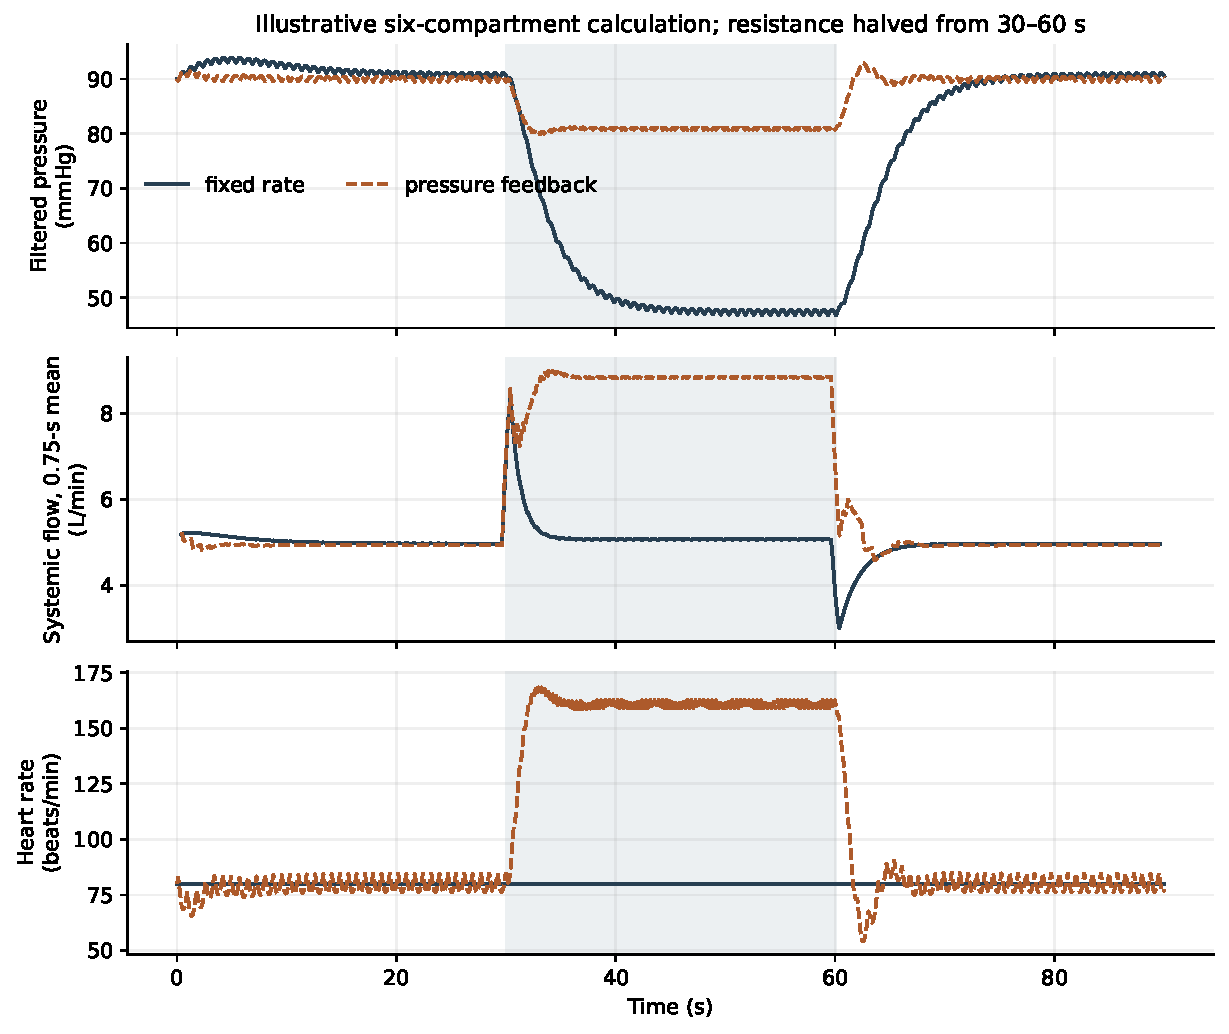
\includegraphics[width=.96\linewidth,height=.57\textheight,keepaspectratio]{feedback-response.pdf}\par\smallskip
{\small Original calculation from demo.py with Rs 17.86 $\to$ 8.93 $\to$ 17.86 mmHg min/L, transitions at 30 and 60 s, reference rate 80 beats/min, target 90 mmHg and filter time 3 s. Fixed rate is compared with gain 10 feedback bounded at 30--240 beats/min. Shading marks reduced resistance. Systemic flow has a centered 0.75 s display average. Default step: 0.00046875 s (1600 steps per reference beat).}
\end{minipage}\end{center}
\section{Equilibrium offsets and numerical sensitivity}
\hypertarget{note-equilibrium-offsets-and-numerical-sensitivity}{}\label{note:equilibrium-offsets-and-numerical-sensitivity}
{\small \href{slides.html\#frame=the-proportional-control-offset\&step=1}{Slides for this section}}\par
Begin verification with claims that have exact structure. The sum of all compartment volumes should remain constant to floating-point tolerance. For each accepted step, the change in each stored volume divided by the step should match net flow. Ideal valve flows must not be negative, and their states must agree with the accepted pressure ordering. With gain zero, the rate must equal the reference rate and the accumulated phase must be a straight line. A deliberately strong target reset should expose any negative unbounded rate command while the declared bound keeps the actual phase increasing.

Then test accuracy against an independently formulated reference. The supplied author test integrates stressed volumes with an adaptive Radau solver over one fixed-rate cycle and compares pressure-step solutions after conversion to those same volume variables. Refining from 200 to 1600 steps per reference beat reduces the maximum discrepancy in that test. This does not establish a universal convergence order for all feedback trajectories or resolve every valve-switching error. Repeat refinement for the observable used in a new scientific claim: cycle means, peak pressure, recovery overshoot or event timing may converge differently.

Cross-language agreement is a separate check. The original MATLAB companion implements the same declared algorithm and accepts the same parameters; a comparison script can check saved Python reference traces. At this author handoff, actual GNU Octave 10.3.0 runs of the refined fixed-rate and feedback protocols pass the declared comparison; MATLAB itself was not run. Matching two implementations would still not prove that their shared equations represent physiology. Distinguish algebraic verification, numerical accuracy, reproduction of a source, and validation against observations.

The feedback default uses 1600 steps per 80-beats/min reference cycle. A coarser 400-step version conserved volume but amplified tiny perturbations enough to spoil long-trajectory agreement between Python and Octave. Refinement reduced that sensitivity, and the refined 90-second feedback traces passed the original absolute comparison tolerance of 0.0001 in each recorded column's units. This is an observed numerical limitation of the tested setup, not evidence of chaotic physiology. The exact forcing grid also avoids artificial, roundoff-sized final steps at event boundaries.

Away from clipping, a steady required rate $F_{\rm req}$ gives
\[
 \frac{P_* -\bar P}{P_*}=\frac{F_{\rm req}/F_0-1}{g}.
\]
Pure proportional feedback therefore needs a nonzero pressure error whenever the regulated operating point requires $F_{\rm req}\ne F_0$. Increasing $g$ reduces this static offset, but the filter and circulation introduce delays that can change transient stability. Rate bounds prevent the proportional formula from demanding an inadmissible clock speed; they do not guarantee accurate or stable dynamics for every gain.
\bigskip
\section*{Exercises}
\par\noindent\begin{minipage}{\linewidth}
\subsection*{E1. An altered resistance: constitutive law versus system response}
Use a new test state with systemic pressures 88 and 4 mmHg and resistance 21 mmHg min/L. This problem is separate from the notebook worked example.

\textbf{a} Calculate flow before and immediately after reducing resistance by one third, holding the two pressures fixed.

\end{minipage}\par\medskip
\textbf{b} Explain why neither that calculation nor fixed heart rate determines the eventual cardiac output of the closed circuit.

\textbf{c} A program changes resistance and its pressure trace changes, but reported flow remains proportional to the old conductance. Give a targeted test and correction.

\par\noindent\begin{minipage}{\linewidth}
\subsection*{E2. Conservation with changing storage}
A closed compartment has unstressed volume 0.030 L, initial compliance 0.012 L/mmHg, initial pressure 6 mmHg and new compliance 0.008 L/mmHg.

\textbf{a} With no net flow, calculate its new pressure and total volume.

\end{minipage}\par\medskip
\textbf{b} Prove conservation of total blood volume for the fixed-valve matrix update, stating the matrix property you use.

\textbf{c} Can a six-compartment step pass that conservation test while its valves are wrong? Explain an additional acceptance check.

\par\noindent\begin{minipage}{\linewidth}
\subsection*{E3. A clock that cannot run backward}
Use a reference rate of 75 beats/min, target 100 mmHg, gain 4, current filtered pressure 110 mmHg, arterial pressure 90 mmHg, tau 2 s, step 0.02 s and model bounds 30--200 beats/min.

\textbf{a} Compute one Euler filter update, the rate command, the bounded rate and the cycle-phase increment.

\end{minipage}\par\medskip
\textbf{b} After a target reset, suppose the updated filtered pressure is 135 mmHg while the target is again 100 mmHg. Compute the unbounded and bounded rates and explain what should be reported.

\textbf{c} For a differentiable varying rate F(t), differentiate the tempting definition phase =\allowbreak{} tF(t) and compare it with the intended clock equation.

\par\noindent\begin{minipage}{\linewidth}
\subsection*{E4. Design a defensible recovery comparison}
An investigator says that waiting one filter time before any recovery change must minimize peak pressure. You may design computations but need not perform a parameter sweep.

\textbf{a} Define two distinct delay protocols and one shared comparison metric, including the time window.

\end{minipage}\par\medskip
\textbf{b} Specify numerical checks needed before ranking the protocols.

\textbf{c} State one conclusion the comparison could support and one it could not support.

\section*{References}
\noindent\begin{minipage}{\linewidth}
Zan Ahmad, Advanced Topics in Computational Cardiology syllabus, Fall 2024. PDF pages 1--2.

\end{minipage}\par\medskip
\noindent\begin{minipage}{\linewidth}
Original EN.500.111 Project 1: feedback control of the circulation. PDF pages 1--3; especially Problem 2 on page 2.

\end{minipage}\par\medskip
\noindent\begin{minipage}{\linewidth}
Hoppensteadt and Peskin, Modeling and Simulation in Medicine and the Life Sciences, second edition. Printed pages 48--51 and 55--58 (supplied PDF pages 61--64 and 68--71); printed page 21, Table 1.3.

\end{minipage}\par\medskip
\noindent\begin{minipage}{\linewidth}
Zan Ahmad and Charles S. Peskin, Continuously Varying Heart Rate in a Pulsatile Circulation Model with Feedback Control. Current 21-page version: pages 2--7, 11, and 18--20; equations (29) and (31).

\end{minipage}\par\medskip
\end{document}
